\documentclass{article}

\usepackage[utf8]{inputenc}
\usepackage[b4paper, margin=1in]{geometry}
\usepackage{booktabs}
\usepackage{graphicx}

\newcommand{\RomanNumeralCaps}[1]
    {\MakeUppercase{\romannumeral #1}}

\title{Data Exercise Notes}
\author{Saksham Kaushal}


\begin{document}
	\maketitle
	
	\section{Photometry}
	\begin{enumerate}
		
		\item \textbf{Do you understand what is changing?} -- using \emph{autocut, colour map, intensity map,} and \emph{colour bar}.
		
		\item \textbf{How can you determine which object is the nova?}
		
		Using multiple images. Nova are transients with their luminosities fading over time, typically few days/weeks. So, looking out for stars with luminosities fading over time would help us determine which object is a nova.
		\(\alpha = 00:44:41.05, \delta = 40:08:36.00\)
		
		\item \textbf{Header contents, position and pixel information}
		
		\begin{table} [h] 
			\centering
			\begin{tabular}[width=\linewidth] {l r r r r r}
				\toprule
				\textbf{file} & \textbf{DATE-OBS} & \textbf{MJD} & \textbf{EXPTIME} & \textbf{AIRMASS} & \textbf{x-axis span} \\
				\midrule
				phot\_00.fits & 2016/07/16 01:54:04.626 & 57585.079220 & 120 & 1.7258910 & 1049--1061 \\
				phot\_01.fits & 2016/07/17 01:57:55.414 & 57586.081891 & 120 & 1.6665240 & 1049--1061 \\
				phot\_02.fits & 2016/07/18 01:43:20.318 & 57587.071763 & 120 & 1.7491860 & 1049--1061 \\
				phot\_03.fits & 2016/07/19 01:36:39.439 & 57588.067123 & 120 & 1.7721150 & 1050--1061 \\
				phot\_04.fits & 2016/07/22 02:34:57.627 & 57591.107611 & 120 & 1.3530670 & 1052--1058 \\
				phot\_05.fits & 2016/07/25 01:29:33.555 & 57594.062194 & 120 & 1.6443790 & 1053--1058 \\
				phot\_06.fits & 2016/07/27 01:35:03.477 & 57596.066012 & 120 & 1.5562500 & 1052--1058 \\
				phot\_07.fits & 2016/08/03 03:15:00.354 & 57603.135421 & 120 & 1.1115970 & 1053--1058 \\
				phot\_08.fits & 2016/08/09 01:19:45.090 & 57609.055383 & 120 & 1.3717510 & 1050--1060 \\
				phot\_09.fits & 2016/08/17 01:26:10.686 & 57617.059846 & 120 & 1.2355820 & 1053--1058 \\
				phot\_10.fits & 2016/08/19 02:09:48.268 & 57619.090142 & 120 & 1.1156090 & 1053--1058 \\
				phot\_11.fits & 2016/08/21 02:53:30.765 & 57621.120495 & 120 & 1.0482370 & --- \\
				phot\_12.fits & 2016/08/27 01:30:12.240 & 57627.062642 & 120 & 1.1306350 & 1053--1057 \\
				phot\_13.fits & 2016/08/29 03:01:21.059 & 57629.125938 & 120 & 1.0244450 & 1054--1057 \\
				phot\_14.fits & 2016/09/06 02:28:01.479 & 57637.102795 & 120 & 1.0250930 & 1054--1057 \\
				phot\_15.fits & 2016/09/13 23:52:30.836 & 57644.994801 & 120 & 1.1904340 & 1054--1056 \\
				phot\_16.fits & 2016/09/24 02:27:20.058 & 57655.102315 & 300 & 1.0329910 & 1053--1056 \\
				phot\_17.fits & 2016/09/28 02:53:32.834 & 57659.120519 & 300 & 1.0706010 & 1054--1056 \\
				\bottomrule
			\end{tabular}
		\end{table}
		GAIN = 1.62, Position = (1055,978) for all entries. 
		
		\item \textbf{Are the number of pixels containing light from the nova (i.e. the point spread function or PSF) the
			same in every image? What two effects could be changing this?}
		
		No. Change in auto-cut value and variations in brightness of background or nova can change the viewed psf.
		
		\item \textbf{Why is it important to do this?} -- enter \emph{exposure time} and \emph{gain} for each observation.
		
		Image of a faint object captured over long exposure time may be brighter than the image of a bright object captured over smaller exposure time. Similarly, high gain would require more photons per data unit. Therefore, for different values of gain too, our perception of bright and faint objects may vary from one image to another. Hence, it is important to account for exposure time and gain for each image.
		
		\item \textbf{Why would it be undesirable to use an aperture that is either too small or too large?}
		
		A very small aperture would lead to loss of signal by disacrding useful signal. A large aperture would include a lot of noise. Hence in both cases, signal to noise ratio is decreased, although in different ways. An optimal aperture considers all the signal while discarding maximum possible noise. In aperture photometry, the outer annulus is used to account for calculate average noise value. This value is subtracted from the aperture signal to obtain true signal. If the aperture contains noise (very large aperture) or discards signal (very small aperture), the calculated value will account for smaller than true overall value of signal or signal to noise ratio. 
		
		\item \textbf{Signal to noise ratios for different apertures. How do you decide which aperture is optimal?}
		
		\begin{table} [h]
			\centering
			\begin{tabular} {r r r r r r}
				\toprule
				\textbf{radius} & \textbf{magnitude} &\textbf{mag error} & \textbf{signal} & \textbf{noise} &\textbf{SNR} \\
				\midrule
				6.0 & -8.02378 & 0.00512 & 3656.2 & 1620.0 & 2.257 \\
				10.4 & -8.13224 & 0.00738 & 3629.6 & 1790.2 & 2.0275 \\
				15.5 & -8.15562 & 0.01047 & 3627.2 & 1829.1 & 1.983 \\
				26.5 & -8.16615 & 0.01745 & 3626.2 & 1847.0 & 1.963 \\
				\bottomrule
			\end{tabular}
		\end{table}
		
		Optimal is systematically decided using data count results instead of magnitude results. A rough estimate for better understanding can be performed using table above.
		
		\item \textbf{Do the results you have obtained, by varying the aperture size, vary randomly as you might expect with measurement error?}
		
		No. Results vary in a well defined manner according to the reasons stated above. The errors are not random, and instead depend upon the radius of the aperture. Both small and large apertures are inefficient and an optimum aperture lies in between that range.
		
		\item \textbf{determine the optimal aperture size.}
		
		\begin{table} [h]
			\centering
			\begin{tabular} {l r r r}
				\toprule
				\textbf{aperture (semi-major axis)} & \textbf{mean counts} & \textbf{error in counts} & \textbf{SNR}\\
				\midrule
				3.0 & 36.784 & 0.10739 & 342.527 \\
				4.0 & 26.835 & 0.037792 & 710.071 \\
				5.0 & 19.433 & 0.024469 & 794.189 \\
				6.0 & 14.398 & 0.016884 & 852.760 \\
				7.0 & 11.029 & 0.013013 & 847.537 \\
				8.0 & 8.6644 & 0.011412 & 759.236 \\
				9.0 & 6.9651 & 0.010593 & 657.519 \\
				10.0 & 5.7077 & 0.010112 & 564.448 \\
				11.0 & 4.7566 & 0.0094432 & 503.706 \\
				12.0 & 4.0395 & 0.0089313 & 452.286 \\
				13.0 & 3.4646 & 0.0082037 & 422.322 \\
				14.0 & 2.9852 & 0.0072329 & 412.725 \\
				15.0 & 2.6030 & 0.0066956 & 388.763 \\
				16.0 & 2.2916 & 0.0062298 & 367.845 \\
				17.0 & 2.0352 & 0.0057338 & 354.948 \\
				18.0 & 1.8190 & 0.0054112 & 336.155 \\
				19.0 & 1.6286 & 0.0051199 & 318.092 \\
				20.0 & 1.4728 & 0.0048525 & 303.514 \\
				25.0 & 0.94289 & 0.0039804 & 236.883 \\
				\bottomrule
			\end{tabular}
		\end{table}
		\(r_a=1.5\) and \(r_b=2.0\). SNR = [342.527,710.071,794.189,852.760,847.537,759.236, 657.519, 564.448, 503.706, 452.286, 422.322, 412.725, 388.763, 367.845, 354.948, 336.155, 318.092, 303.514]
		
		\begin{figure}[h]
			\centering
			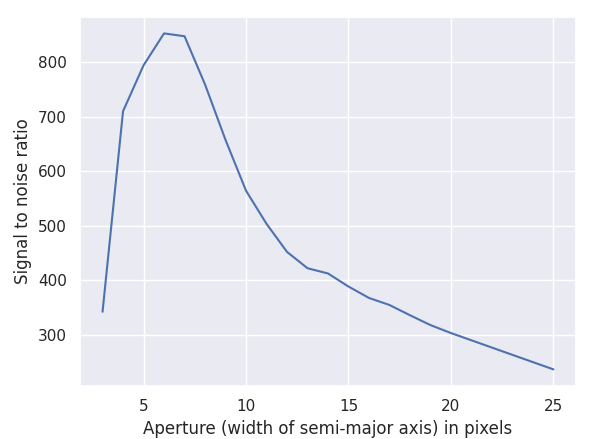
\includegraphics[width=.7\linewidth]{../codes/plots/optimal_aperture_phot_00.png}
		\end{figure}
		
		
		\item \textbf{What would be the effect of changing the aperture size between measurements within the same image?}
		
		Would give inconsistent values of magnitudes for different objects.  
		
		\item \textbf{Optimal apertures for all images.}
		\begin{table}[h]
			\centering
			\begin{tabular} {l r}
				\toprule
				\textbf{file} & \textbf{aperture} \\
				\midrule
				00 & 7.0 \\
				01 & 6.5 \\
				02 & 5.5 \\
				03 & 5.4 \\
				04 & 4.9 \\
				05 & 4.9 \\
				06 & 8.0 \\
				07 & 4.4 \\
				08 & 7.5 \\
				09 & 4.6 \\
				10 & 3.1 \\
				11 & 4.4 \\
				12 & 3.6 \\
				13 & 2.5 \\
				14 & 2.3 \\
				15 & 4.2 \\
				16 & 3.3 \\
				17 & 2.9 \\
				\bottomrule
			\end{tabular}
		\end{table}
		
		\item \textbf{Does the optimal aperture size vary between the images? If so, what causes this?}
		
		Optimal aperture size varies for different images depending upon atmospheric seeing (or the background noise), exposure time, object brightness, etc.
		
		\item \textbf{Why does this approach work?
What problems might be associated with this method?} -- using secondary stars for photometry.
		
		We need to consider only the stars which have been observed to remain static (i.e. not a variable star) over extremely long periods, so that its low photometric uncertainty can be considered reliable for calibration. If such a non-variable star lies in our field of view while observing the science object, the photometry of that object can be calibrated using the nearby secondary standard. Even if the atmospheric conditions are not very favourable, photometry can still be performed if we can safely assume that the extent of unfavourability of conditions is similar for both the objects, which is a reasonable assumption for nearby secondary standards. Secondly, widely separated secondary stars in the field of view can be used to estimate variability in atmospheric extinction across field of view. For faint events, exposure times are long and many of the primary standards appear saturated. Dimmer secondary stars therefore are more helpful in these cases.
		
		 \item \textbf{How can we determine which of the PS1 stars might be suitable to use?}
		
		Vicinity to the nova and comparable brightness. Vicinity would lead to correlating atmospheric extinction values, which would be roughly similar for all, and therefore, easily accounted for. Similar brightness or \emph{spread} of stars would aid the use of same aperture for all standard stars and nova in the image. Also, every secondary star selected should be properly resolved in the image.
		
		\item \textbf{Secondary stars}
		
		ID = [11,2,6,30,10]
		
		\item \textbf{Photometry of nova and stars}
		
		\begin{table} [h]
			\centering
			\begin{tabular} {l r r r r r r}
				\toprule
				\textbf{image} & \textbf{nova} & \textbf{star 1 (1079,741)} & \textbf{star 2 (985,665)} & \textbf{star 3 (740,1205)} & \textbf{star 4 (392,1111)} & \textbf{star 5 (1275,1305)} \\
				\midrule
				00 & -8.06917,0.00554 & -8.79153,0.00311 & -8.19322,0.00501 & -8.43167,0.00413 & -6.81993,0.01639 & -9.23457,0.00222 \\
				01 & -8.11788,0.00477 & -9.08614,0.00228 & -8.49188,0.00355 & -8.72659,0.00296 & -7.11721,0.01104 & -9.52156,0.00168 \\
				02 & -7.78778,0.00655 & -8.94943,0.00261 & -8.34755,0.00414 & -8.58463,0.00344 & -6.95411,0.01345 & -9.37925,0.00192 \\
				03 & -7.7492,0.00711 & -9.06624,0.00248 & -8.47205,0.00392 & -8.70987,0.00324 & -7.09267,0.1257 & -9.50961,0.0018 \\
				04 & -7.01378,0.01582 & -8.67234,0.00379 & -8.0789,0.00621 & -8.32961,0.00501 & -6.72892,0.02037 & -9.10936,0.00268 \\
				05 & -6.7958,0.01559 & -8.76096,0.00302 & -8.16958,0.00477 & -8.41133,0.00394 & -6.80057,0.01552 & -9.20142,0.00218 \\
				06 & -6.22505,0.02621 & -8.4437,0.0039 & -7.86253,0.00628 & -8.09466,0.00516 & -6.45922,0.02131 & -8.86995,0.00281 \\
				07 & -6.00348,0.00998 & -8.78424,0.00191 & -8.19902,0.00259 & -8.44785,0.00226 & -6.83937,0.00566 & -9.23819,0.00152 \\
				08 & -5.19026,0.03097 & -8.44701,0.00266 & -7.86816,0.00381 & -8.10531,0.00328 & -6.48753,0.01046 & -8.89045,0.00205 \\
				09 & -5.31643,0.04588 & -9.07027,0.0021 & -8.47533,0.00321 & -8.72066,0.00267 & -7.124,0.00931 & -9.51246,0.00158 \\
				10 & -4.58417,0.07163 & -8.58765,0.00271 & -8.00687,0.00403 & -8.26852,0.00333 & -6.63258,0.01166 & -9.03455,0.00204 \\
				11 & 0.351068,0.28434 & -7.62915,0.00734 & -7.06545,0.01171 & -7.29312,0.00969 & -5.63848,0.04075 & -8.08902,0.00511 \\
				12 & -4.08713,0.03827 & -8.71743,0.00193 & -8.13829,0.00256 & -8.38544,0.00226 & -6.7756,0.00543 & -9.16339,0.00156 \\
				13 & -3.75681,0.03747 & -8.40337,0.00228 & -7.81135,0.00305 & -8.07205,0.00267 & -6.45187,0.00618 & -8.85114,0.00185 \\
				14 & -3.27988,0.05617 & -8.46164,0.00225 & -7.89683,0.00291 & -8.15279,0.00256 & -6.5255,0.00592 & -8.93343,0.00178 \\
				15 & -3.37124,0.19267 & -8.81852,0.00219 & -8.2141,0.00324 & -8.4636,0.00275 & -6.86197,0.00885 & -9.25069,0.00169 \\
				16 & -2.69049,0.10301 & -8.5127,0.00143 & -7.91725,0.00196 & -8.17252,0.0017 & -6.53396,0.00448 & -8.95882,0.00114 \\
				17 & -1.99732,0.1288 & -8.08944,0.0018 & -7.49395,0.00242 & -7.76262,0.00208 & -6.09845,0.00533 & -8.51768,0.00149 \\
				\bottomrule
			\end{tabular}
		\end{table}
	
		\item \textbf{Catalog entries SDSS conversions.}
		\begin{table} [h]
			\centering
			\begin{tabular} {l r r r r r}
				\toprule
				\textbf{ID} & \textbf{r} & \textbf{r error} & \textbf{g} & \textbf{g error} & \textbf{r'} \\
				\midrule
				2 (1079,741) & 16.1868 & 0.0044 & 16.8984 & 0.0052 & 16.194 \\
				6 (985,665) & 16.7696 & 0.0065 & 17.5087 & 0.0059 & 16.777 \\
				10 (740,1205) & 16.5210 & 0.0066 & 16.9415 & 0.0034 & 16.525 \\
				30 (392,1111) & 18.1143 & 0.0062 & 18.5278 & 0.0049 & 18.118\\
				11 (1275,1305)& 15.7283 & 0.0020 & 16.0337 & 0.0042 & 15.731 \\
				\bottomrule
			\end{tabular}
		\end{table}
	
		\item \textbf{Airmass and Z values for each star.}
		\begin{table} [h]
			\centering
			\begin{tabular} {l r r r r r}
				\toprule
				\textbf{airmass} & \textbf{star 1} & \textbf{star 2} & \textbf{star 3} & \textbf{star 4} & \textbf{star 5} \\
				\midrule
				1.7258910 & 24.98553,0.00711 & 24.97022,0.00901 & 24.95667,0.00813 & 24.93793,0.02039 & 15.99236, 0.02636 \\
				1.6665240 & 25.28014,0.00628 & 25.26888,0.00755 & 25.25159,0.00696 & 25.23521,0.01504 & 15.98576, 0.02342 \\
				1.7491860 & 25.14343,0.00661 & 25.12455,0.00814 & 25.10963,0.00744 & 25.07211,0.01745 & 16.25722, 0.02611 \\
				1.7721150 & 25.26024,0.00648 & 25.24905,0.00792 & 25.23487,0.00724 & 25.21067,0.12970 & 16.27953, 0.06946 \\
				1.3530670 & 24.86634,0.00779 & 24.85590,0.01021 & 24.85461,0.00901 & 24.84692,0.02437 & 17.31224, 0.03807 \\
				1.6443790 & 24.95496,0.00702 & 24.94658,0.00877 & 24.93633,0.00794 & 24.91857,0.01952 & 17.32355, 0.03586 \\
				1.5562500 & 24.63770,0.00790 & 24.63953,0.01028 & 24.61966,0.00916 & 24.57722,0.02531 & 17.95682, 0.04862 \\
				1.1115970 & 24.97824,0.00591 & 24.97602,0.00659 & 24.97285,0.00626 & 24.95737,0.00966 & 18.49384, 0.02681 \\
				1.3717510 & 24.64101,0.00666 & 24.64516,0.00781 & 24.63031,0.00728 & 24.60553,0.01446 & 19.12250, 0.04948 \\
				1.2355820 & 25.26427,0.00610 & 25.25233,0.00721 & 25.24566,0.00667 & 25.24200,0.01331 & 19.09294, 0.06365 \\
				1.1156090 & 24.78165,0.00671 & 24.78387,0.00803 & 24.79352,0.00733 & 24.75058,0.01566 & 19.91031, 0.09037 \\
				1.0482370 & 23.82315,0.01134 & 23.84245,0.01571 & 23.81812,0.01369 & 23.75648,0.04475 & 24.89334, 0.31344 \\
				1.1306350 & 24.91143,0.00593 & 24.91529,0.00656 & 24.91044,0.00626 & 24.89360,0.00943 & 20.39669, 0.05496 \\
				1.0244450 & 24.59737,0.00628 & 24.58835,0.00705 & 24.59705,0.00667 & 24.56987,0.01018 & 20.80234, 0.05463 \\
				1.0250930 & 24.65564,0.00625 & 24.67383,0.00691 & 24.67779,0.00656 & 24.64350,0.00992 & 21.27881, 0.07318 \\
				1.1904340 & 25.01252,0.00619 & 24.99110,0.00724 & 24.98860,0.00675 & 24.97997,0.01285 & 21.07015, 0.21031 \\
				1.0329910 & 24.70670,0.00543 & 24.69425,0.00596 & 24.69752,0.00570 & 24.65196,0.00848 & 21.86260, 0.11905 \\
				1.0706010 & 24.28344,0.00580 & 24.27095,0.00642 & 24.28762,0.00608 & 24.21645,0.00933 & 22.52909, 0.14532 \\
				\bottomrule
			\end{tabular}
		\end{table}
		
		\item \textbf{Z at airmass 1 for secndary stars.}
		\begin{table}[h]
			\centering
			\begin{tabular} {l r r}
				\toprule
				\textbf{star} & \textbf{Z at airmass 1} & \textbf{slope} \\
				\midrule
				1 & 24.58518 & 0.72978 \\
				2 & 24.58542 & 0.71267 \\
				3 & 24.58767 & 0.68760 \\
				4 & 24.55271 & 0.70689 \\
				5 & 24.57150 & 0.71021\\
				\bottomrule
			\end{tabular}
		\end{table}
		
		\item \textbf{Photometric measurements of nova using different standard stars.}
		\begin{table} [h]
			\centering
			\begin{tabular} {l r r r r r r}
				\toprule
				\textbf{image} & \textbf{star 1} & \textbf{star 2} & \textbf{star 3} & \textbf{star 4} & \textbf{star 5} & \textbf{mean}\\
				\midrule
				00 & 15.98627, 0.02225 & 15.99893, 0.02695 & 16.01938, 0.02367 & 15.97041, 0.03703 & 15.98679, 0.01796 & 15.99236, 0.12786 \\
				01 & 15.98088, 0.02065 & 15.99253, 0.02472 & 16.01149, 0.02173 & 15.96367, 0.03091 & 15.98025, 0.01665 & 15.98576, 0.11466 \\
				02 & 16.25066, 0.02276 & 16.26372, 0.02709 & 16.28475, 0.02399 & 16.23534, 0.03510 & 16.25164, 0.01867 & 16.25722, 0.12761 \\
				03 & 16.27250, 0.02319 & 16.28596, 0.02743 & 16.30756, 0.02435 & 16.25771, 0.14791 & 16.27393, 0.01911 & 16.27953, 0.24199 \\
				04 & 17.31374, 0.03321 & 17.32002, 0.03843 & 17.33112, 0.03483 & 17.28935, 0.05129 & 17.30697, 0.02870 & 17.31224, 0.18646 \\
				05 & 17.31912, 0.03221 & 17.33039, 0.03676 & 17.34879, 0.03353 & 17.30140, 0.04621 & 17.31805, 0.02797 & 17.32355, 0.17668 \\
				06 & 17.95419, 0.04371 & 17.96394, 0.04889 & 17.98014, 0.04537 & 17.93445, 0.06262 & 17.95139, 0.03922 & 17.95682, 0.23981 \\
				07 & 18.50026, 0.02549 & 18.50240, 0.02897 & 18.50745, 0.02624 & 18.47034, 0.03074 & 18.48876, 0.02170 & 18.49384, 0.13314 \\
				08 & 19.12362, 0.04723 & 19.13022, 0.05118 & 19.14179, 0.04825 & 19.09966, 0.05653 & 19.11722, 0.04322 & 19.12250, 0.24641 \\
				09 & 19.09683, 0.06158 & 19.10109, 0.06549 & 19.10925, 0.06255 & 19.06975, 0.07029 & 19.08776, 0.05766 & 19.09294, 0.31757 \\
				10 & 19.91664, 0.08794 & 19.91885, 0.09206 & 19.92400, 0.08896 & 19.88682, 0.09839 & 19.90522, 0.08387 & 19.91031, 0.45122 \\
				11 & 24.90104, 0.30528 & 24.90211, 0.31245 & 24.90557, 0.30803 & 24.86968, 0.34019 & 24.88831, 0.29965 & 24.89334, 1.56560 \\
				12 & 20.40271, 0.05380 & 20.40519, 0.05723 & 20.41071, 0.05453 & 20.37323, 0.05880 & 20.39159, 0.05003 & 20.39669, 0.27439 \\
				13 & 20.81053, 0.05335 & 20.81118, 0.05692 & 20.81405, 0.05414 & 20.77862, 0.05875 & 20.79733, 0.04952 & 20.80234, 0.27268 \\
				14 & 21.28699, 0.07202 & 21.28765, 0.07548 & 21.29053, 0.07273 & 21.25509, 0.07719 & 21.27380, 0.06815 & 21.27881, 0.36557 \\
				15 & 21.07496, 0.20846 & 21.07846, 0.21231 & 21.08549, 0.20942 & 21.04685, 0.21662 & 21.06501, 0.20456 & 21.07015, 1.05137 \\
				16 & 21.87061, 0.11804 & 21.87141, 0.12137 & 21.87449, 0.11871 & 21.83890, 0.12259 & 21.85758, 0.11435 & 21.86260, 0.59506 \\
				17 & 22.53634, 0.14420 & 22.53778, 0.14762 & 22.54180, 0.14488 & 22.50548, 0.14923 & 22.52404, 0.14049 & 22.52909, 0.72642 \\
				\bottomrule
			\end{tabular}
		\end{table}

	\end{enumerate}

% ================================ Spectroscopy ==========================================
	\clearpage
	
	\section{Spectroscopy}
	\begin{enumerate}

		\item \textbf{Do you understand what these units (particularly those for the y-axis) are telling you?} \\
		The spectrum obtained is a plot of power per unit area, per unit wavelength (flux density) as a function of wavelength, which essentially tells us the distribution of energy as a function of wavelength.

		\item \textbf{Do you know what an ‘erg’ is?} \\
		An \emph{erg} is a unit of energy. Numerically, \(1 \textrm{erg} = 10^{-7} \textrm{Joules}\).

		\item \textbf{Can you identify all five components?} \\
		Yes. the continuum emission from the nova, emission lines formed within the nova ejecta, absorption lines from the interstellar medium, cosmic rays, and statistical noise. 

		\item \textbf{Do you understand how they each arise?} \\
		Continuum emission from thermal radiations emitted over a large wavelength range by the inner dense material. \\
		Emission lines from radiation emitted by surrounding ejecta which absorbs wavelengths from continuum and emits at specific wavelengths. \\
		Absortion lines from radiation absorbed by the column of ISM in our line of sight of nova. \\
		Cosmic rays of galactic, extra-galactic and solar origins. \\
		Statistical noise inherent to measurements from instruments. Also called shot noise, it doesn't have any fixed pattern.

		\item \textbf{The emission lines in these spectra are all ‘recombination lines’. Do you know how such emission lines and the interstellar absorption lines form?} \\
		Emission recombination lines form when an ion captures a free electron. The electron is captured at higher energy levels of the ion and then \emph{cascades} down to lower energy levels, thereby emitting at multiple wavelengths. \\
		ISM absorption lines are formed due to absorption of specific wavelength by cold gas of extremely low density. Dust containing metals also absorbs certain wavelengths depending upon the metals contained in the grains.

		\item \textbf{However, you should notice that the cosmic rays contained within each spectrum are in different places, do you understand why this is?} \\
		Two components which are random for each exposure are the cosmic ray hits and statistical noises. 

		\item \textbf{Why might multiple exposures be advantageous over a single observation?} \\
		This prevents saturation. Leads to fewer cosmic ray hits and noise due to transient moving objects in the sky (asteroids, satellites, etc.). Multiple exposures can be used to remove random defects.

		\item \textbf{Are there any disadvantages associated with multiple exposures?} \\
		Slight increase in readout noise.

		\item \textbf{Do you understand how such an approach can lead to the removal of most (if not all) cosmic rays from a set of images/spectra?} \\
		Median of (at least) three values would remove cosmic ray hits given that they are at different locations for each exposure. This is unlike statistical noise is present in each exposure at every wavelength.

		\item \textbf{How do each the five components of the spectra (as determined in the previous section) change with time?} \\
		Continuum emission - reduced in strength over time. More quickly in the earlier spectra.\\
		Emission lines - reduced in strength over time. More quickly in the earlier spectra. Some weaker emissions fade completely over time. \\
		ISM absorption is stronger when continuum emission is stronger. With passing time absorption fades. \\
		Cosmic Rays - Remain constant, but their occurence has been removed from spectra upon taking median for each epoch. \\
		Statistical noise increases very slightly as we go to later spectra. SNR value reduces with time.

		\item \textbf{What effect has the stacking process had upon these spectra, has it been completely successful?} \\
		Stacking removed cosmic ray hits almost entirely. Statistical noise, however, has not seen improvement. All other components have been preserved although extremely small signals may now seem lost in the statistical noise.

		\item \textbf{Can the spectra be displayed in a more suitable fashion?} \\
		Yes, once it's known that the strength of continuum reduced over time, it can be removed for comparing evolutions of line emissions.

		\item \textbf{Using Table 3, identify each line and determine the spectroscopic class of this particular nova.}
		The lines observed are H \textsc{\romannumeral 1} (H \textsc{\(\delta\)}, H \textsc{\(\gamma\)}, H \textsc{\(\beta\)}, H \textsc{\(\alpha\)}), Fe \textsc{\romannumeral 2} (42,48,49), O \textsc{\romannumeral 1} (1,21,55) and possibly Si \textsc{\romannumeral 2} (4). The nova is of Fe \textsc{\romannumeral 2} spectroscopic class.

		\item \textbf{Can you devise a test, using the continuum fitting function, to ascertain whether you have successfully subtracted the continuum?} \\
		Once the continuum has been fit, try fitting it once again. This time the new fitting curve should be a horizontal line corresponding to zero flux density. This would imply that the continuum has been fit.

		\item \textbf{Continuum flux, line flux, equivalent width and E(B--V)} \\
		\begin{table} [h]
			\centering
			\begin{tabular} {l r r r r r}
				\toprule
				\textbf{central wavelength} & \textbf{continuum flux} & \textbf{line flux} & \textbf{EW} & \textbf{log[E(B--V)]} & \textbf{E(B--V)} \\
				\midrule
				\(5890.009\pm 0.061\) & \(2.400 \times 10^{-16} \pm 1.5068 \times 10^{-17}\) & \(-1.345 \times 10^{-16} \pm 1.143 \times 10^{-16}\) & 0.560 & \(-0.700 \pm 0.15\) & \(0.199 \pm 0.069\) \\
				\(5895.935 \pm 0.175\) & \(2.402 \times 10^{-16} \pm 1.5068 \times 10^{-17}\) & \(-9.309 \times 10^{-17} \pm 1.263 \times 10^{-16}\) & 0.388 & \(-0.802 \pm 0.17\) & \(0.158 \pm 0.062\) \\
				\bottomrule
			\end{tabular}
		\end{table}

		Average value of E(B--V) = \(0.1785 \pm 0.093\).

		\item \textbf{Measure the flux and FWHM of all the Balmer (H }\textsc{\RomanNumeralCaps 1} \textbf{) lines, plus at least one line from another species.} \\
		\begin{table}
			\centering
			\begin{tabular} {l r}
				\toprule
				\midrule
				\bottomrule
			\end{tabular}
		\end{table}


	\end{enumerate}
\end{document}	